\documentclass[tekniskrapport/tech.tex]{subfiles}

\begin{document}

\section{Kommunikationsmodul}
Kommunikationsmodulen styr bilen och kommunicerar med fjärrklienten.
Sensorvärden från sensormodulen tolkas av kommunikationsmodulen som därefter
skickar felvärden till styrmodulen.

Bildbehandling utförs av kommunikationsmodulen för att
avgöra bilens position i vägfilen och upptäcka stopplinjer. Med hjälp av
kamerans bilder på vägen skapas ett felvärde som kan användas för att justera
taxins riktning.

Kommunikation med fjärrklienten sköts av kommunikationsmodulen för
att skicka sensorvärden och annan relevant information. Modulen tar
även emot uppdrag.

Autonomitet utförs av kommunikationsmodulen för att utföra uppdraget.
Kommunikationsmodulen hämtar sensordata från sensormodulen och bildbehandlar
kamerabilderna för att utföra beslut i realtid. Besluten skickas i form av fel-
och styrvärden till styrmodulen.

Kommunikationsmodulens program är skriven i både C och C++. Bildbehandlingen är
skriven i C++ medan resten av programmet är implementerad med C. De olika
delarna kompileras separat och länkas sedan ihop med kompilatorn för C++.
Programmet består av tre trådar; en huvudtråd som hanterar uppdrag och
bildbehandlar, samt en tråd som sköter kommunikation via SPI och en som svarar
på kommandon från fjärrklienten via TCP/IP. SPI:n och servern sköts i separata
trådar eftersom de väntar mycket och blockerar den nuvarande tråden.


\subsection{Hårdvaruimplementation} 
Kommunikationsmodulen har implementerats i en Raspberry Pi 3B. Raspberry Pi 3B,
har en fyrkärnig processor med en hastighet på 1.2 GHz vilket har kunnat
utnyttjas inte minst vid bildbehandlingen. Med 40-pinnar som kan utnyttjas som
spänningskällor, jord, programmerbara GPIO-portar samt seriella bussar, har
detta utnyttjats för att med SPI-protokollet använda Raspberry Pi:n som master
för två slavar. Då kommunikationen med en fjärrklient sker via WiFi har det
inbyggda 802.11n trådlösa LAN:et varit fullt kapabelt. Det trådlösa
nätverkskortet hade med en bra implementation även kunnat strömma video. Mitt
på Pi:en hittar man en CSI-port som används för att ansluta Raspberry Pi
kompatibla kameror. Kameran som används på kommunikations modulen är en
Raspberry Pi kamera med påsatt vidvinkelobjektiv som kan se i en 160 graders vy.
Kameran har även stöd för två infrarödastrålkastare, men detta används inte då
mörkerseende inte är något som prioriterats. Spänningskällor finns i både 3V3
och 5V.

\paragraph{Programstruktur}
Programmet på kommandomodulen består av följande filer

\begin{labeling}{wwww}
    \item[server.c] Server som anropar kommandofunktioner vid förfrågan från
        klient från separat tråd.
	\item[spi.c] Lågnivåfunktioner för SPI.
    \item[bus.c] Hantering av SPI-buss, utför kommandon på bussen och anropar
        signalhanterare från separat tråd.
    \item[ip/img\_proc.cpp] Bildbehandling med OpenCV.
    \item[objective.c] Utförarande av uppdrag.
    \item[main.c] Huvudloop och implementation av signalhanterare för buss och
        server.
\end{labeling}

\paragraph{Huvudtråden} startar servern och busshanteraren. Därefter startar
den huvudloopen som antingen tar styrvärden utifrån användarens kommandon via
servern eller från uppdragshanteraren med hjälp av bildbehandling. Därefter schemaläggs
skrivning av de nya styrvärdena till styrmodulen. Dessutom schemaläggs hämtning
av sensorvärden från sensorerna.

\paragraph{Server}
% TODO

\paragraph{Busshanterare} 
% TODO

\subsection{Bildbehandling}
% TODO
\paragraph{Upptäkt av linjer}

\paragraph{Tolkning av linjer}

\subsection{Uppdrag}

\begin{wrapfigure}{r}{0.3\linewidth}
    \begin{center}
        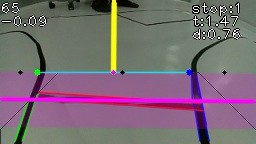
\includegraphics[width=\linewidth]{tekniskrapport/figures/opencv.jpg}
    \end{center}
    \caption{Klassificering och tolkning av linjer från kamera.}
\end{wrapfigure}

\subsubsection{Uppdrag} \label{sec:comm-mission}
% TODO
För att utföra uppdraget kommer en kö av kommandon tas emot från fjärrklienten.
När uppdraget börjar kör taxin framåt och följer filen med hjälp av
bildbehandling och reglering. Inför varje stopplinje tas ett kommando från kön
och utförs. Om ett hinder upptäcks under uppdraget kommer bilen att stanna
tills hindret har försvunnit eller eventuellt passera hindret. När ett visst
antal stopplinjer har passerats och kön är tom är uppdraget avklarat. Nedan är
en lista av alla möjliga kommandon hur de utförs.
\begin{labeling}{wwww}
    \item[\commIgnore] Kör förbi stopplinjen utan att stanna.
    \item[\commStop] Stanna framför stopplinjen, fortsätt efter några sekunder
    om kön inte är tom.
    \item[\commPark] Parkera i fickan till höger efter stopplinjen, lämna
    parkeringen och fortsätt efter några sekunder om kön inte är tom.
    \item[\commEnter] Sväng höger in i rondellen och hitta rondellens körfil.
    \item[\commContinue] Kör förbi stopplinje och håll till vänster.
    \item[\commExit] Sväng höger ut ur rondellen och hitta körfilen.
\end{labeling}

\end{document}
